\documentclass[11pt,letterpaper]{article}
\usepackage[utf8]{inputenc}

%----- Configuración del estilo del documento------%
\usepackage{epsfig,graphicx}
\usepackage[left=2cm,right=2cm,top=1.8cm,bottom=2.3cm]{geometry}
\usepackage{fancyhdr}
\usepackage{lastpage}
\usepackage{url}
\pagestyle{fancy}
\fancyhf{}
\rfoot{\textit{Página \thepage \hspace{1pt} de \pageref{LastPage}}}


%------ Paquetes matemáticos básicos --------%
\usepackage{amsmath}
\usepackage{amssymb}
\usepackage{amsthm}

\usepackage[spanish]{babel}
\usepackage{graphicx}
\usepackage{hyperref}

\usepackage{tabularx}
\usepackage{xcolor}
\usepackage[table]{xcolor}
\usepackage{colortbl}
\usepackage{array, multirow, multicol, tabularx}
\usepackage{tcolorbox}
\newtheorem{theorem}{Theorem}[section]
\newtheorem{corollary}{Corollary}[theorem]
\newtheorem{lemma}[theorem]{Lemma}

%------si-------%
\definecolor{B}{HTML}{FFFFFF}
\definecolor{G}{HTML}{5e5e5e}
\definecolor{R2}{HTML}{d53d40}
\definecolor{A2}{HTML}{034190}
\definecolor{V2}{HTML}{7faa50}
\newcommand{\R}{\mathbb{R}}
\newcommand{\C}{\mathcal{C}}
\newcommand{\N}{\mathbb{N}}
\newcommand{\Z}{\mathbb{Z}}
\newcommand{\Q}{\mathbb{Q}}
\renewcommand{\theenumi}{\Roman{enumi}}
\renewcommand{\labelenumi}{{\theenumi}.}

\begin{document}

%------ Encabezado -------- %

\begin{center}
    \begin{minipage}{3cm}
    	\begin{center}
    		\includegraphics[height=3.4cm]{logo_unam.png}
    	\end{center}
    \end{minipage}\hfill
    \begin{minipage}{10cm}
    	\begin{center}
    	\textbf{\large Universidad Nacional Autónoma de México}\\[0.1cm]
        \textbf{Facultad de Ciencias}\\[0.1cm]
        \textbf{C\'alculo II}\\[0.1cm]
        Decima extra\\[0.1cm]
         El\'ias L\'opez Rivera\\[0.1cm]
        \texttt{ elias.lopezr\,@ciencias.unam.mx }\\[0.1cm]
        Fecha:\,\,25/04/2025
    	\end{center}
    \end{minipage}\hfill
    \begin{minipage}{3cm}
    	\begin{center}
    		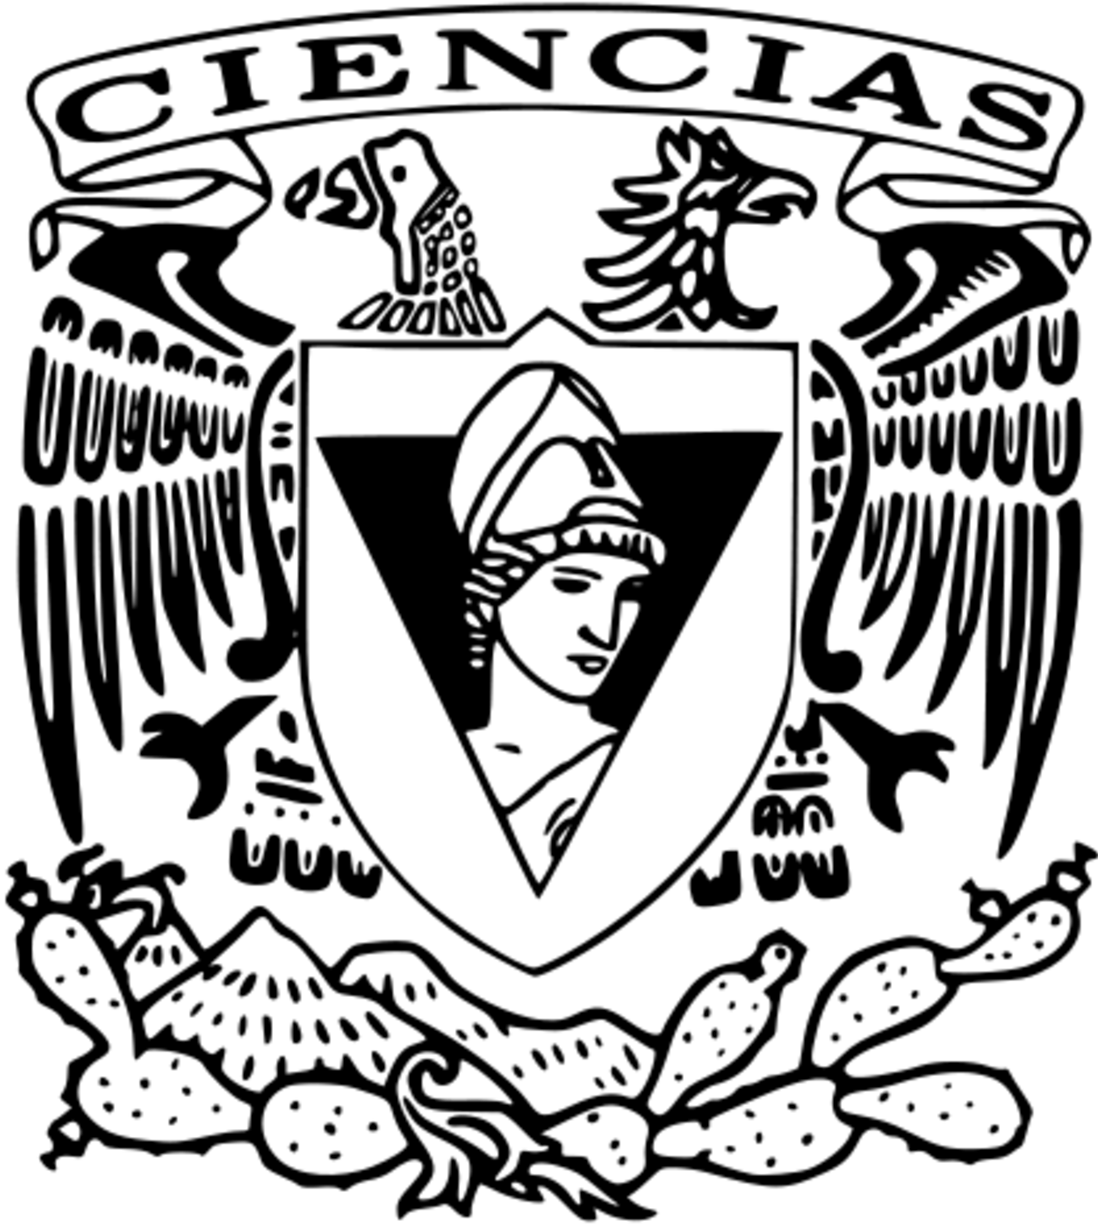
\includegraphics[height=3.4cm]{Logo_FC.png}
    	\end{center}
    \end{minipage}
\end{center}

\rule{17cm}{0.1mm}

%------ Fin de encabezado -------- %
\,\\
\begin{tcolorbox}[
	title = \textcolor{black}{\textcolor{white}{Problema}},]
\textit{Encuentre el siguiente l\'imite\,\\
\begin{equation*}
\displaystyle\lim_{x\rightarrow\,0}\,\frac{3(\,(\log(x+1)-3x+\frac{3}{2}x^2)^5\,(6\sen(x^2)+65x^6-6x^2)^{\frac{5}{6}})}{x^3e^{x^2}\,((1+\sen(x))^x-1+\pi x)(\cos(\sen(x^3))-1)}
\end{equation*}
}
\end{tcolorbox}\,\\
\begin{proof}\,\\
Procederemos a abordar el l\'imite por polinomios de Taylor, por tanto reestringimos $|x|\leq 1$, y comenzamos a acotar:\,\\
    \,\\
    \textbf{I})\,\,$f(x)=\cos(\sen(x^3))$
\end{proof}\,\\
Recordamos que la composici\'on de polinomios de taylor cumple que:\,\\
\,\\
\begin{equation*}
    P_{g\circ r,n,0}=[\,P_{g,n,0}\circ P_{r,n,0}\,]_{n}
\end{equation*}\,\\
Por tanto tenemos que sea $l(x)=\sen(x^3)$ se cumple que:\,\\
\,\\
\begin{equation*}
    P_{l,6,0}=\left[x^3-\frac{x^9}{3!}+\frac{x^{15}}{5!}\right]_{6}=x^3
\end{equation*}\,\\
Luego tenemos que:\,\\
\,\\
\begin{equation*}
    P_{f,6,0}=\left[1-\frac{x^6}{2!}+\frac{x^{12}}{4!}-\frac{x^{18}}{6!}\right]_{6}=1-\frac{x^6}{2!}
\end{equation*}\,\\
Finalmente obtenemos que:\,\\
\begin{equation*}
    f(x)=1-\frac{x^6}{2!}+R_{f,6,0}
\end{equation*}\,\\
\,\\
\textbf{II)}\,\,$z(x)=sen(x^2)$\,\\
\,\\
Tenemos que:\,\\
\,\\
\begin{equation*}
    P_{z,6,0}=\left[x^2-\frac{x^6}{3!}+\frac{x^{15}}{5!}\right]_{6}=x^2-\frac{x^6}{3!}
\end{equation*}\,\\
Por tanto\,\\
\,\\
\begin{equation*}
    z(x)=x^2-\frac{x^6}{3!}+R_{z,6,0}
\end{equation*}\,\\
\textbf{III)}\,\,$w(x)=log(x+1)$\,\\
\,\\
Como reestringimos $-1<x\leq 1$, tenemos que:\,\\
\,\\
\begin{equation*}
    w(x)=x+R_{w,1,0}
\end{equation*}\,\\
\,\\
\textbf{IV)}\,\,$g(x)=e^{xlog(1+sen(x))}$\,\\
\,\\
Definimos $c(x)=log(1+sen(x))$, como $-1\leq sen(x)\leq1$, tenemos que:\,\\
\,\\
\begin{equation*}
    P_{c,1,0}=[x]_{1}=x
\end{equation*}\,\\
Luego recordando que el polinomio de grado $n$ de una multiplicaci\'on es la multiplicaci\'on
de los correspondientes polinomios de grado $n$ truncada a solo los grados menores o iguales a $n$,tenemos que
\,\\
\,\\
\begin{equation*}
    P_{xc,1,0}=[x^2]_{1}=0
\end{equation*}\,\\
Finalmente usando de nuevo el teorema de composici\'on\,\\
\,\\
\begin{equation*}
    P_{g,1,0}=[1]_{1}=1
\end{equation*}\,\\
Por tanto\,\\
\,\\
\begin{equation*}
    g(x)=1+R_{g,1,0}
\end{equation*}\,\\
\newpage
\,\\
Ahora reescribimos el l\'imite con \textbf{I),II),III),IV)}\,\\
\,\\
\begin{equation*}
    \displaystyle\lim_{x\rightarrow\,0}\,\frac{3(\,(-2x+\frac{3}{2}x^2+R_{w,1,0})^5\,(6x^2-x^6+6R_{z,6,0}+65x^6-6x^2)^{\frac{5}{6}})}{x^3e^{x^2}\,(\pi x+R_{g,1,0})(R_{f,6,0}-\frac{x^6}{2!})}
\end{equation*}\,\\
Reduciendo y factorizando el l\'imite\,\\
\,\\
\begin{equation*}
    \displaystyle\lim_{x\rightarrow\,0}\,\frac{3\left(\,x^5\left(-2+\frac{3}{2}x+\frac{R_{w,1,0}}{x}\right)^5\,x^5\left(6\frac{R_{z,6,0}}{x^6}+64\right)^{\frac{5}{6}}\right)}{x^3e^{x^2}\,x\left(\pi +\frac{R_{g,1,0}}{x}\right)\,x^6\left(\frac{R_{f,6,0}}{x^6}-\frac{1}{2!}\right)}
\end{equation*}\,\\
Reduciendo a\'un m\'as:\,\\
\,\\
\begin{equation*}
    \displaystyle\lim_{x\rightarrow\,0}\,\frac{3\left(\,\left(-2+\frac{3}{2}x+\frac{R_{w,1,0}}{x}\right)^5\,\left(6\frac{R_{z,6,0}}{x^6}+64\right)^{\frac{5}{6}}\right)}{e^{x^2}\,\left(\pi +\frac{R_{g,1,0}}{x}\right)\,\left(\frac{R_{f,6,0}}{x^6}-\frac{1}{2!}\right)}
\end{equation*}\,\\
\,\\
Usando la propiedad del residuo, y todos los teoremas de l\'imites pertinentes finalmente obtenemos:\,\\
\,\\
\begin{equation*}
    \displaystyle\lim_{x\rightarrow\,0}\,\frac{3(\,(\log(x+1)-3x+\frac{3}{2}x^2)^5\,(6\sen(x^2)+65x^6-6x^2)^{\frac{5}{6}})}{x^3e^{x^2}\,((1+\sen(x))^x-1+\pi x)(\cos(\sen(x^3))-1)}=\frac{(3)(-2)^5(64)^{5/6}}{-\frac{\pi}{2}}=\frac{3(2^{11})}{\pi}
\end{equation*}
\end {document}